\documentclass[twoside]{book}

% Packages required by doxygen
\usepackage{calc}
\usepackage{doxygen}
\usepackage{graphicx}
\usepackage[utf8]{inputenc}
\usepackage{makeidx}
\usepackage{multicol}
\usepackage{multirow}
\usepackage{textcomp}
\usepackage[table]{xcolor}

% Font selection
\usepackage[T1]{fontenc}
\usepackage{mathptmx}
\usepackage[scaled=.90]{helvet}
\usepackage{courier}
\usepackage{amssymb}
\usepackage{sectsty}
\renewcommand{\familydefault}{\sfdefault}
\allsectionsfont{%
  \fontseries{bc}\selectfont%
  \color{darkgray}%
}
\renewcommand{\DoxyLabelFont}{%
  \fontseries{bc}\selectfont%
  \color{darkgray}%
}

% Page & text layout
\usepackage{geometry}
\geometry{%
  a4paper,%
  top=2.5cm,%
  bottom=2.5cm,%
  left=2.5cm,%
  right=2.5cm%
}
\tolerance=750
\hfuzz=15pt
\hbadness=750
\setlength{\emergencystretch}{15pt}
\setlength{\parindent}{0cm}
\setlength{\parskip}{0.2cm}
\makeatletter
\renewcommand{\paragraph}{%
  \@startsection{paragraph}{4}{0ex}{-1.0ex}{1.0ex}{%
    \normalfont\normalsize\bfseries\SS@parafont%
  }%
}
\renewcommand{\subparagraph}{%
  \@startsection{subparagraph}{5}{0ex}{-1.0ex}{1.0ex}{%
    \normalfont\normalsize\bfseries\SS@subparafont%
  }%
}
\makeatother

% Headers & footers
\usepackage{fancyhdr}
\pagestyle{fancyplain}
\fancyhead[LE]{\fancyplain{}{\bfseries\thepage}}
\fancyhead[CE]{\fancyplain{}{}}
\fancyhead[RE]{\fancyplain{}{\bfseries\leftmark}}
\fancyhead[LO]{\fancyplain{}{\bfseries\rightmark}}
\fancyhead[CO]{\fancyplain{}{}}
\fancyhead[RO]{\fancyplain{}{\bfseries\thepage}}
\fancyfoot[LE]{\fancyplain{}{}}
\fancyfoot[CE]{\fancyplain{}{}}
\fancyfoot[RE]{\fancyplain{}{\bfseries\scriptsize Generated on Thu Jun 5 2014 14\-:01\-:05 for vw4tools by Doxygen }}
\fancyfoot[LO]{\fancyplain{}{\bfseries\scriptsize Generated on Thu Jun 5 2014 14\-:01\-:05 for vw4tools by Doxygen }}
\fancyfoot[CO]{\fancyplain{}{}}
\fancyfoot[RO]{\fancyplain{}{}}
\renewcommand{\footrulewidth}{0.4pt}
\renewcommand{\chaptermark}[1]{%
  \markboth{#1}{}%
}
\renewcommand{\sectionmark}[1]{%
  \markright{\thesection\ #1}%
}

% Indices & bibliography
\usepackage{natbib}
\usepackage[titles]{tocloft}
\setcounter{tocdepth}{3}
\setcounter{secnumdepth}{5}
\makeindex

% Custom commands
\newcommand{\clearemptydoublepage}{%
  \newpage{\pagestyle{empty}\cleardoublepage}%
}


%===== C O N T E N T S =====

\begin{document}

% Titlepage & ToC
\pagenumbering{roman}
\begin{titlepage}
\vspace*{7cm}
\begin{center}%
{\Large vw4tools \\[1ex]\large 0.\-9-\/1 }\\
\vspace*{1cm}
{\large Generated by Doxygen 1.8.6}\\
\vspace*{0.5cm}
{\small Thu Jun 5 2014 14:01:05}\\
\end{center}
\end{titlepage}
\clearemptydoublepage
\tableofcontents
\clearemptydoublepage
\pagenumbering{arabic}

%--- Begin generated contents ---
\chapter{Java\-Doc A\-P\-I Markup for vw4tools}
\label{index}\section*{vw4tools }

Tools and utilities for Virtual\+Wisdom4

At current, V\+W4\+Tools is a script or two, plus one big jar file. vw4tool.\+jar allows a user to import a text file in one of several formats and output an Entity import J\+S\+O\+N for Virtual\+Wisdom4.

\section*{Running Java }

In this document, it is assumed \char`\"{}java\char`\"{} runs from the command prompt. In some cases, this isn't true. Windows users, for example, may need to change their usage, from\+: \begin{DoxyVerb}java -jar vw4tool.jar ...
\end{DoxyVerb}


to\+: \begin{DoxyVerb}java.exe -jar vw4tool.jar ...
\end{DoxyVerb}


In both cases, if the \char`\"{}java\char`\"{} (or java.\+exe) executable is not available on the user's \char`\"{}path\char`\"{} or list of locations wherein to find a binary/executable, the user will need to type the full pathname to the java executable.

Macintosh O\+S\+X users can simply type \char`\"{}java\char`\"{}\+: \begin{DoxyVerb}java -jar vw4tool.jar ...
\end{DoxyVerb}


A U\+N\+I\+X (or unix-\/like) user may need to type /opt/local/bin/java or similar\+: \begin{DoxyVerb}/opt/local/bin/java -jar vw4tool.jar ...
\end{DoxyVerb}


A Windows user may need to type a full pathname such as\+: \begin{DoxyVerb}"C:\Program Files (x86)\Java\jre7\bin\java.exe" -jar vw4tool.jar ...
\end{DoxyVerb}


In all cases, where I type merely \char`\"{}java\char`\"{}, make sure you replace that with however the invocation details are for your platform.

To confirm you've found a working Java Runtime Environment, use the \char`\"{}help\char`\"{} command to as vw4tool.\+jar what version it is\+: \begin{DoxyVerb}java -jar vw4tool.jar --help
Usage: vw4tool -V|--version|-H|--help
     : vw4tool --read <filename>|--input <filename> | -r <filename> | -i <filename>
   ie: vw4tool --read import.json
   ie: vw4tool -r import.json
\end{DoxyVerb}


note\+: many commands have shorter versions. \char`\"{}-\/-\/version\char`\"{} (with two \char`\"{}-\/\char`\"{}) is the same as \char`\"{}-\/\+V\char`\"{} (with one dash). Pay special attention to case. Uppercase \char`\"{}\+N\char`\"{} is different from lowercase \char`\"{}n\char`\"{}.

\section*{Common Usage }

\begin{DoxyVerb}java -jar vw4tool.jar  -N localfile1.txt -N localfile2.txt -N localfile3.txt -oexample.json
\end{DoxyVerb}


or \begin{DoxyVerb}java -jar vw4tool.jar  -N localfile1.txt -N localfile2.txt -N localfile3.txt -oOrderedTuples.csv
awk -f csv-to-json.awk OrderedTuples.csv > example.json
\end{DoxyVerb}


This is the most common usage, here as a reference. Notice that although this shows E\+I\+T\+H\+E\+R Ordered\+Tuples.\+csv or a J\+S\+O\+N file being created, both could be created by multiple \char`\"{}-\/o\char`\"{} options. Notice also that although in past, \char`\"{}-\/o\char`\"{} was \char`\"{}cuddled\char`\"{} to the filename after it (no spaces), but this has changed to make it easier and more forgiving to use.

\section*{Overview }

In general, collection and conversion looks like the following diagram\+:

\begin{center}

\begin{DoxyImageNoCaption}
  \mbox{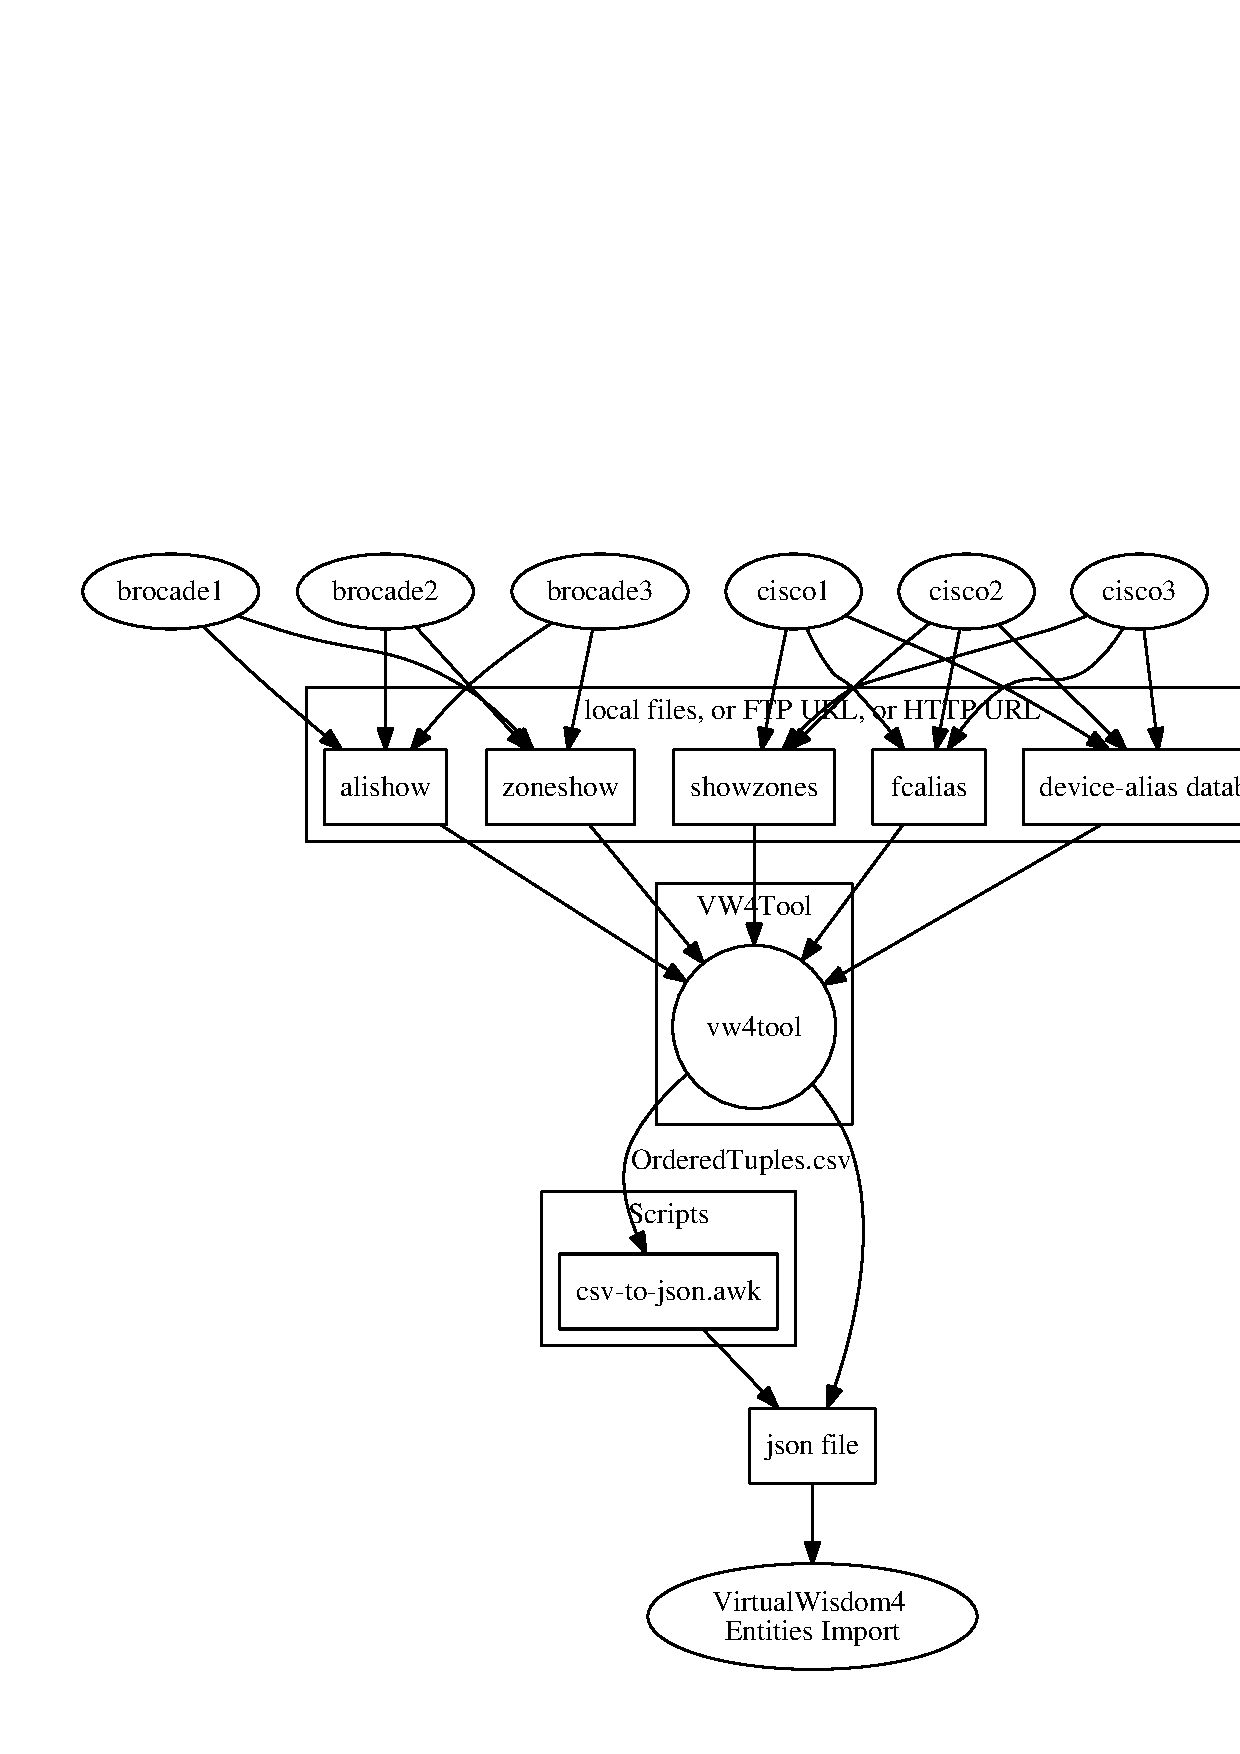
\includegraphics[width=\textwidth,height=\textheight/2,keepaspectratio=true]{dot_inline_dotgraph_1}}
\end{DoxyImageNoCaption}
\end{center}


\section*{Import of F\+T\+P or H\+T\+T\+P Data }

V\+W4\+Tools uses the U\+R\+L\+Data\+Source functionality to open a stream from a H\+T\+T\+P or F\+T\+P server; this means that the files it parses can be stored on a local filesystem, a F\+T\+P server, and an H\+T\+T\+P server as constant data, or can be the result of a C\+G\+I program on an H\+T\+T\+P server. Less common, a local file may also be mounted as a F\+U\+S\+E filesystem, allowing even \char`\"{}local\char`\"{} data to be generated like a C\+G\+I program.

In order to draw a text stream from a F\+T\+P server or H\+T\+T\+P server, merely use a R\+F\+C-\/1738-\/compliant U\+R\+L to indicate these two sources\+: \begin{DoxyVerb}(ftp|http)://{user{:password@@}server{:port}/pathname/to/resource
\end{DoxyVerb}


for example\+:

(basic user/pass\+: user = scott, pass = T1ger, host = ftp.\+example.\+com, subdir = . , file = nicknames.\+txt \begin{DoxyVerb}java -jar vw4tool.jar --nickname=ftp://scott:T1ger@@ftp.example.com/nicknames.txt
\end{DoxyVerb}


(basic user/pass\+: user = scott, pass = T1ger, host = ftp.\+example.\+com, subdir = /users/local/\+Scott\+Adams/ , file = aliases.\+text \begin{DoxyVerb}java -jar vw4tool.jar --nickname=ftp://scott:T1ger@@ftp.example.com/%2fusers/local/ScottAdams/aliases.text
\end{DoxyVerb}


(basic user/pass\+: user = anonymous, pass = scott@uberserver.\+net, host = ftp.\+example.\+com, subdir = examples , file = aliases \begin{DoxyVerb}java -jar vw4tool.jar -N ftp://anonymous:scott%2Fuberserver.net@@ftp.example.com/examples/aliases
\end{DoxyVerb}


(basic http\+: host = www.\+example.\+com, subdir = . , file = aliases \begin{DoxyVerb}java -jar vw4tool.jar --nickname=http://www.example.com/aliases
\end{DoxyVerb}


(basic H\+T\+T\+P G\+E\+T\+: host = www.\+example.\+com, subdir = . , path=/cgi-\/bin/fetch.cgi, some parameters \begin{DoxyVerb}java -jar vw4tool.jar --nickname=http://www.example.com/cgi-bin/fetch.cgi?now=20140901&realm=WEST&group=production
\end{DoxyVerb}


N\+O\+T\+E\+: \char`\"{}-\/-\/nickname=\char`\"{} and \char`\"{}-\/\+N\char`\"{} are functionally identical; \char`\"{}-\/-\/nickname=\char`\"{} may offer a slight beefit in more clearly self-\/documenting the behavior of the commandline option.

\section*{Import of Local Text File }

The most common usage is local text files representing the metadata of the local environment. This is done by offering a R\+F\+C-\/1738-\/compliant local file U\+R\+L\+: \begin{DoxyVerb}file://pathname/to/resource
\end{DoxyVerb}


Note that if the \char`\"{}file\+://\char`\"{} is not given, and no \char`\"{}protocol\char`\"{} (ie \char`\"{}file\+://\char`\"{}) is given, vw4tool will warn you about this but try the local {\tt file\+://} protocol prefix for you

for example\+:

(local file in subdir ./files/aliases) \begin{DoxyVerb}java -jar vw4tool.jar --nickname=file://files/aliases
java -jar vw4tool.jar --nickname=files/aliases
\end{DoxyVerb}


(local file in subdir /\+Full/\+Path/files/aliases) \begin{DoxyVerb}java -jar vw4tool.jar --nickname=file:///Full/Path/files/aliases
java -jar vw4tool.jar --nickname=/Full/Path/files/aliases
\end{DoxyVerb}


\section*{Specifying Formats }

The user doesn't need to speficy the format of a file; vw4tool will try the file at the same time across many different parsers and see which one can make sense of it. Unfortunately, the parsers cannot always chew through any user-\/interface codes (such as \char`\"{}press any key to continue\char`\"{}) and preamble (the verbose text trash before the actual zone or aliases or such). Trimming that to a minimum offers a better chance of parsing the file.

The corollary to this is that if a file doesn't seem to parse, yet it seems like it should, remove anything before or after the actual content, and confirm that it was collected in a non-\/interactive method. If the user ever needs to \char`\"{}press any key for more\char`\"{}, chances are, the parsed result will be either partial, or none at all.

\section*{Multiple Inputs }

These input formats can be mixed. For example \begin{DoxyVerb}java -jar vw4tool.jar --nickname=http://www.example.com/cgi-bin/fetch.cgi?now=20140901&realm=WEST&group=production -N local.txt -N file:///Users/allanc/aliases.dad -N morefiles.txt
\end{DoxyVerb}


\section*{Outputs }

vw4tool will either generate an Ordered\+Tuples.\+csv file (if that specific filename is given on the \char`\"{}-\/o\char`\"{} option) or a json file (any other putput filename). Or both\+: \begin{DoxyVerb}java -jar vw4tool.jar  -N local.txt -oOrderedTuples.csv -oexample.json
\end{DoxyVerb}


N\+O\+T\+E\+: giving no filename used to send the output to stdout, but now requires a \char`\"{}-\/\char`\"{} to mean \char`\"{}yes, I meant that\char`\"{}\+: \begin{DoxyVerb}java -jar vw4tool.jar  -N local.txt -o -
\end{DoxyVerb}


For this reason, the following two commands used to do different things, but are now equivalent\+: \begin{DoxyVerb}java -jar vw4tool.jar  -N local.txt -oexample.json
java -jar vw4tool.jar  -N local.txt -o example.json
\end{DoxyVerb}


\section*{Proprietary Intellectual Property }

With the exception of samples/import01.\+json, all files and content are based on the same level of access to the product enjoyed by a customer. Implicitly, no private information is shared, all of this content (save the one file) is based on empirical discovery, and could change overnight. 
\chapter{R\-E\-A\-D\-M\-E}
\label{md_htdocs_README}
\input{md_htdocs_README}
\chapter{Data Structure Index}
\section{Data Structures}
Here are the data structures with brief descriptions\-:\begin{DoxyCompactList}
\item\contentsline{section}{{\bf V\-W\-Import.\-Edit\-\_\-\-Type} \\*The edit type of a J\-S\-O\-N for V\-W4 Import can be either \char`\"{}add\char`\"{} or \char`\"{}modify\char`\"{}; the creator needs to know ahead of time whether an entry of the same name currently exists }{\pageref{enumorg_1_1smallfoot_1_1vw4_1_1VWImport_1_1Edit__Type}}{}
\item\contentsline{section}{{\bf V\-W\-Import.\-Entity} \\*An entity for import }{\pageref{classorg_1_1smallfoot_1_1vw4_1_1VWImport_1_1Entity}}{}
\item\contentsline{section}{{\bf Entity} \\*An \doxyref{Entity}{p.}{classorg_1_1smallfoot_1_1vw4_1_1Entity} is the core mutable object used in the J\-S\-O\-N import for V\-W4 }{\pageref{classorg_1_1smallfoot_1_1vw4_1_1Entity}}{}
\item\contentsline{section}{{\bf Entity\-F\-A} \\*An \doxyref{Entity\-F\-A}{p.}{classorg_1_1smallfoot_1_1vw4_1_1EntityFA} is the representation of an Storage F\-A entity in the J\-S\-O\-N import for V\-W4 }{\pageref{classorg_1_1smallfoot_1_1vw4_1_1EntityFA}}{}
\item\contentsline{section}{{\bf Entity\-H\-B\-A} \\*An \doxyref{Entity\-H\-B\-A}{p.}{classorg_1_1smallfoot_1_1vw4_1_1EntityHBA} is the representation of an H\-B\-A entity in the J\-S\-O\-N import for V\-W4 }{\pageref{classorg_1_1smallfoot_1_1vw4_1_1EntityHBA}}{}
\item\contentsline{section}{{\bf Entity.\-Improper\-Child\-Exception} \\*Descendents of \doxyref{Entity}{p.}{classorg_1_1smallfoot_1_1vw4_1_1Entity} should know whether a given entity can be one of their child elements }{\pageref{classorg_1_1smallfoot_1_1vw4_1_1Entity_1_1ImproperChildException}}{}
\item\contentsline{section}{{\bf V\-W\-Import.\-I\-T\-L\-Pattern} \\*An \doxyref{I\-T\-L\-Pattern}{p.}{classorg_1_1smallfoot_1_1vw4_1_1VWImport_1_1ITLPattern} is used to define an application \doxyref{Entity}{p.}{classorg_1_1smallfoot_1_1vw4_1_1VWImport_1_1Entity} based on the I\-T\-Ls it requires }{\pageref{classorg_1_1smallfoot_1_1vw4_1_1VWImport_1_1ITLPattern}}{}
\item\contentsline{section}{{\bf V\-W\-Import.\-Leaf\-Pattern} \\*An \doxyref{Leaf\-Pattern}{p.}{classorg_1_1smallfoot_1_1vw4_1_1VWImport_1_1LeafPattern} is used to define an \doxyref{Entity}{p.}{classorg_1_1smallfoot_1_1vw4_1_1VWImport_1_1Entity} by reference in another entity's child\-\_\-entities }{\pageref{classorg_1_1smallfoot_1_1vw4_1_1VWImport_1_1LeafPattern}}{}
\item\contentsline{section}{{\bf Virtual\-Wisdom4\-Client\-Tool} \\*\doxyref{Virtual\-Wisdom4\-Client\-Tool}{p.}{classorg_1_1smallfoot_1_1vw4_1_1VirtualWisdom4ClientTool} is a \char`\"{}\-Swiss Army Knife\char`\"{} of tools used when working with Virtual\-Wisdom4 }{\pageref{classorg_1_1smallfoot_1_1vw4_1_1VirtualWisdom4ClientTool}}{}
\item\contentsline{section}{{\bf V\-W\-Import} \\*A \doxyref{V\-W\-Import}{p.}{classorg_1_1smallfoot_1_1vw4_1_1VWImport} is a single idempotent import for the Virtual\-Wisdom4 product }{\pageref{classorg_1_1smallfoot_1_1vw4_1_1VWImport}}{}
\end{DoxyCompactList}

\chapter{File Index}
\section{File List}
Here is a list of all documented files with brief descriptions\+:\begin{DoxyCompactList}
\item\contentsline{section}{java/{\bf Entity.\+java} }{\pageref{Entity_8java}}{}
\item\contentsline{section}{java/{\bf Entity\+F\+A.\+java} }{\pageref{EntityFA_8java}}{}
\item\contentsline{section}{java/{\bf Entity\+H\+B\+A.\+java} }{\pageref{EntityHBA_8java}}{}
\item\contentsline{section}{java/{\bf Virtual\+Wisdom4\+Client\+Tool.\+java} }{\pageref{VirtualWisdom4ClientTool_8java}}{}
\item\contentsline{section}{java/{\bf V\+W\+Import.\+java} }{\pageref{VWImport_8java}}{}
\end{DoxyCompactList}

\chapter{Data Structure Documentation}
\section{V\+W\+Import.\+Edit\+\_\+\+Type Enum Reference}
\label{enumorg_1_1smallfoot_1_1vw4_1_1VWImport_1_1Edit__Type}\index{V\+W\+Import.\+Edit\+\_\+\+Type@{V\+W\+Import.\+Edit\+\_\+\+Type}}


The edit type of a J\+S\+O\+N for V\+W4 Import can be either \char`\"{}add\char`\"{} or \char`\"{}modify\char`\"{}; the creator needs to know ahead of time whether an entry of the same name currently exists.  


\subsection*{Data Fields}
\begin{DoxyCompactItemize}
\item 
{\bf add}\label{enumorg_1_1smallfoot_1_1vw4_1_1VWImport_1_1Edit__Type_a393e4cd5187ecf30d2db2129a73f3c05}

\begin{DoxyCompactList}\small\item\em add this element\+: no current element exists with the same name \end{DoxyCompactList}\item 
{\bf modify}\label{enumorg_1_1smallfoot_1_1vw4_1_1VWImport_1_1Edit__Type_afa21b51665d4dc82669bba18a62d8b58}

\begin{DoxyCompactList}\small\item\em use this value to modify an existing element with the same name \end{DoxyCompactList}\end{DoxyCompactItemize}


\subsection{Detailed Description}
The edit type of a J\+S\+O\+N for V\+W4 Import can be either \char`\"{}add\char`\"{} or \char`\"{}modify\char`\"{}; the creator needs to know ahead of time whether an entry of the same name currently exists. 

Definition at line 24 of file V\+W\+Import.\+java.



The documentation for this enum was generated from the following file\+:\begin{DoxyCompactItemize}
\item 
java/{\bf V\+W\+Import.\+java}\end{DoxyCompactItemize}

\section{V\-W\-Import.\-Entity Class Reference}
\label{classorg_1_1smallfoot_1_1vw4_1_1VWImport_1_1Entity}\index{V\-W\-Import.\-Entity@{V\-W\-Import.\-Entity}}


An entity for import.  




Collaboration diagram for V\-W\-Import.\-Entity\-:\nopagebreak
\begin{figure}[H]
\begin{center}
\leavevmode
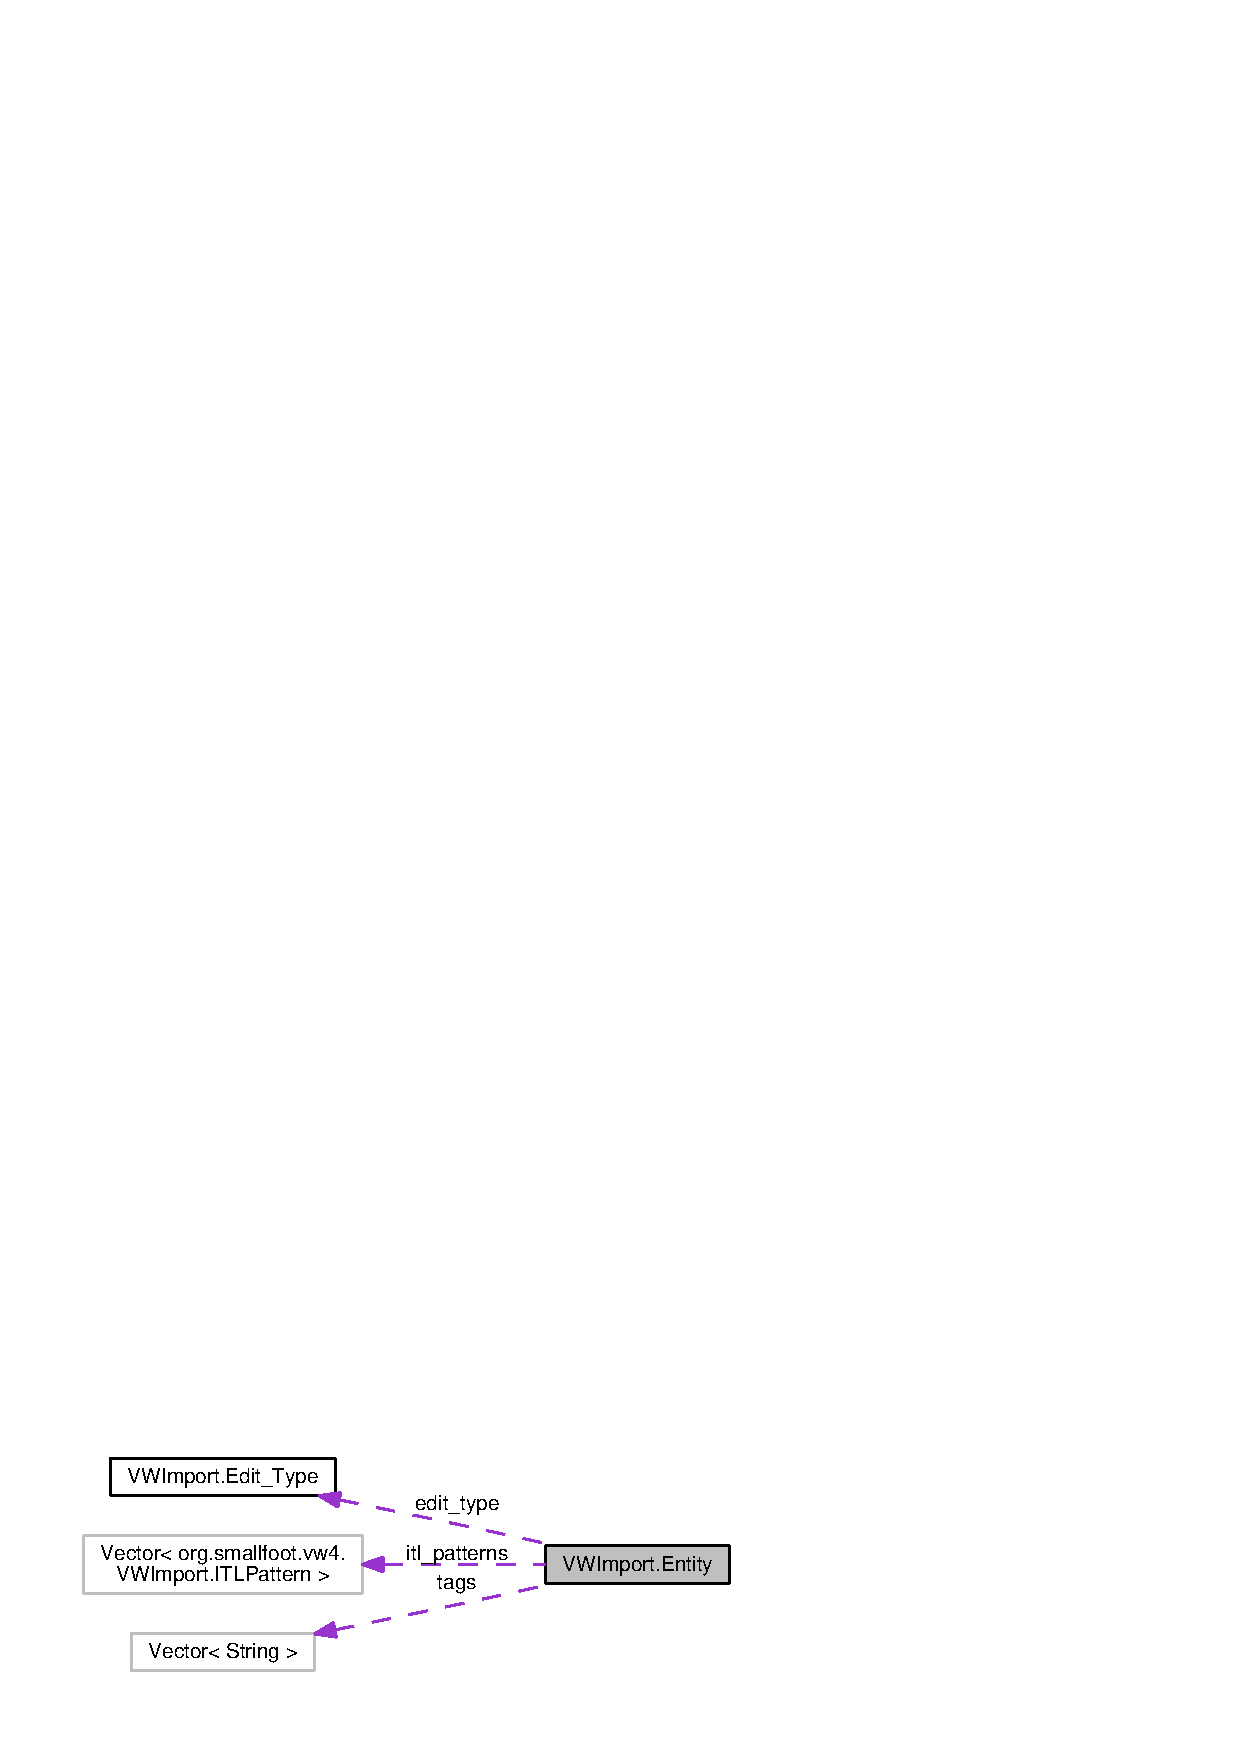
\includegraphics[width=350pt]{classorg_1_1smallfoot_1_1vw4_1_1VWImport_1_1Entity__coll__graph}
\end{center}
\end{figure}
\subsection*{Public Member Functions}
\begin{DoxyCompactItemize}
\item 
Vector$<$ {\bf I\-T\-L\-Pattern} $>$ {\bfseries getitl\-\_\-patterns} ()\label{classorg_1_1smallfoot_1_1vw4_1_1VWImport_1_1Entity_ad56904318d0b6b82c74f21c180c20c86}

\item 
Vector$<$ String $>$ {\bfseries gettags} ()\label{classorg_1_1smallfoot_1_1vw4_1_1VWImport_1_1Entity_a7bd476e2ab1263de941e590ea1e6e97c}

\item 
Vector$<$ {\bf I\-T\-L\-Pattern} $>$ {\bf itl\-\_\-patterns} ()\label{classorg_1_1smallfoot_1_1vw4_1_1VWImport_1_1Entity_abf0e0c927e408646f190445003c49a60}

\begin{DoxyCompactList}\small\item\em singleton access to itl\-\_\-patterns \end{DoxyCompactList}\end{DoxyCompactItemize}
\subsection*{Data Fields}
\begin{DoxyCompactItemize}
\item 
String {\bf description}\label{classorg_1_1smallfoot_1_1vw4_1_1VWImport_1_1Entity_a76d2b0133d83c43dfd8a19286ac55325}

\begin{DoxyCompactList}\small\item\em user-\/readable description f the entity; constraints unknown \end{DoxyCompactList}\item 
{\bf Edit\-\_\-\-Type} {\bf edit\-\_\-type}\label{classorg_1_1smallfoot_1_1vw4_1_1VWImport_1_1Entity_a76dab48266f34c941c947433ae14176d}

\begin{DoxyCompactList}\small\item\em What kind of edit are we doing? Add or Modify? \end{DoxyCompactList}\item 
String {\bfseries name}\label{classorg_1_1smallfoot_1_1vw4_1_1VWImport_1_1Entity_a9a2326f35466e54c36c070829245c557}

\item 
Vector$<$ String $>$ {\bf tags}
\begin{DoxyCompactList}\small\item\em tags for the entity which can be used to define multiple groupings for a given entity. \end{DoxyCompactList}\item 
String {\bf type}\label{classorg_1_1smallfoot_1_1vw4_1_1VWImport_1_1Entity_a0b86e44425dbe3c9d866aa273f87828a}

\begin{DoxyCompactList}\small\item\em What type of \doxyref{Entity}{p.}{classorg_1_1smallfoot_1_1vw4_1_1VWImport_1_1Entity} is this? (full range of values unknown) \end{DoxyCompactList}\end{DoxyCompactItemize}
\subsection*{Protected Attributes}
\begin{DoxyCompactItemize}
\item 
Vector$<$ {\bf I\-T\-L\-Pattern} $>$ {\bf itl\-\_\-patterns}\label{classorg_1_1smallfoot_1_1vw4_1_1VWImport_1_1Entity_a88540be4d74409418ead7a4a7bdc8cee}

\begin{DoxyCompactList}\small\item\em is an \doxyref{Entity}{p.}{classorg_1_1smallfoot_1_1vw4_1_1VWImport_1_1Entity} is defined by I\-T\-L\-Patterns, they would be listed herein \end{DoxyCompactList}\end{DoxyCompactItemize}


\subsection{Detailed Description}
An entity for import. 

Definition at line 46 of file V\-W\-Import.\-java.



\subsection{Field Documentation}
\index{org\-::smallfoot\-::vw4\-::\-V\-W\-Import\-::\-Entity@{org\-::smallfoot\-::vw4\-::\-V\-W\-Import\-::\-Entity}!tags@{tags}}
\index{tags@{tags}!org::smallfoot::vw4::VWImport::Entity@{org\-::smallfoot\-::vw4\-::\-V\-W\-Import\-::\-Entity}}
\subsubsection[{tags}]{\setlength{\rightskip}{0pt plus 5cm}Vector$<$String$>$ tags}\label{classorg_1_1smallfoot_1_1vw4_1_1VWImport_1_1Entity_aa96ebc81ca3bd65e0d7c5e67e96bb973}


tags for the entity which can be used to define multiple groupings for a given entity. 

Better than folders\-: if folders were used, an entity might have only one hierarchical \char`\"{}folder\char`\"{} in which it exists, but any number of tags may be applied to an entity at a time 

Definition at line 49 of file V\-W\-Import.\-java.



The documentation for this class was generated from the following file\-:\begin{DoxyCompactItemize}
\item 
java/{\bf V\-W\-Import.\-java}\end{DoxyCompactItemize}

\section{V\-W\-Import.\-I\-T\-L\-Pattern Class Reference}
\label{classorg_1_1smallfoot_1_1vw4_1_1VWImport_1_1ITLPattern}\index{V\-W\-Import.\-I\-T\-L\-Pattern@{V\-W\-Import.\-I\-T\-L\-Pattern}}


An \doxyref{I\-T\-L\-Pattern}{p.}{classorg_1_1smallfoot_1_1vw4_1_1VWImport_1_1ITLPattern} is udes to define an application \doxyref{Entity}{p.}{classorg_1_1smallfoot_1_1vw4_1_1VWImport_1_1Entity} based on the I\-T\-Ls it requires.  




Collaboration diagram for V\-W\-Import.\-I\-T\-L\-Pattern\-:\nopagebreak
\begin{figure}[H]
\begin{center}
\leavevmode
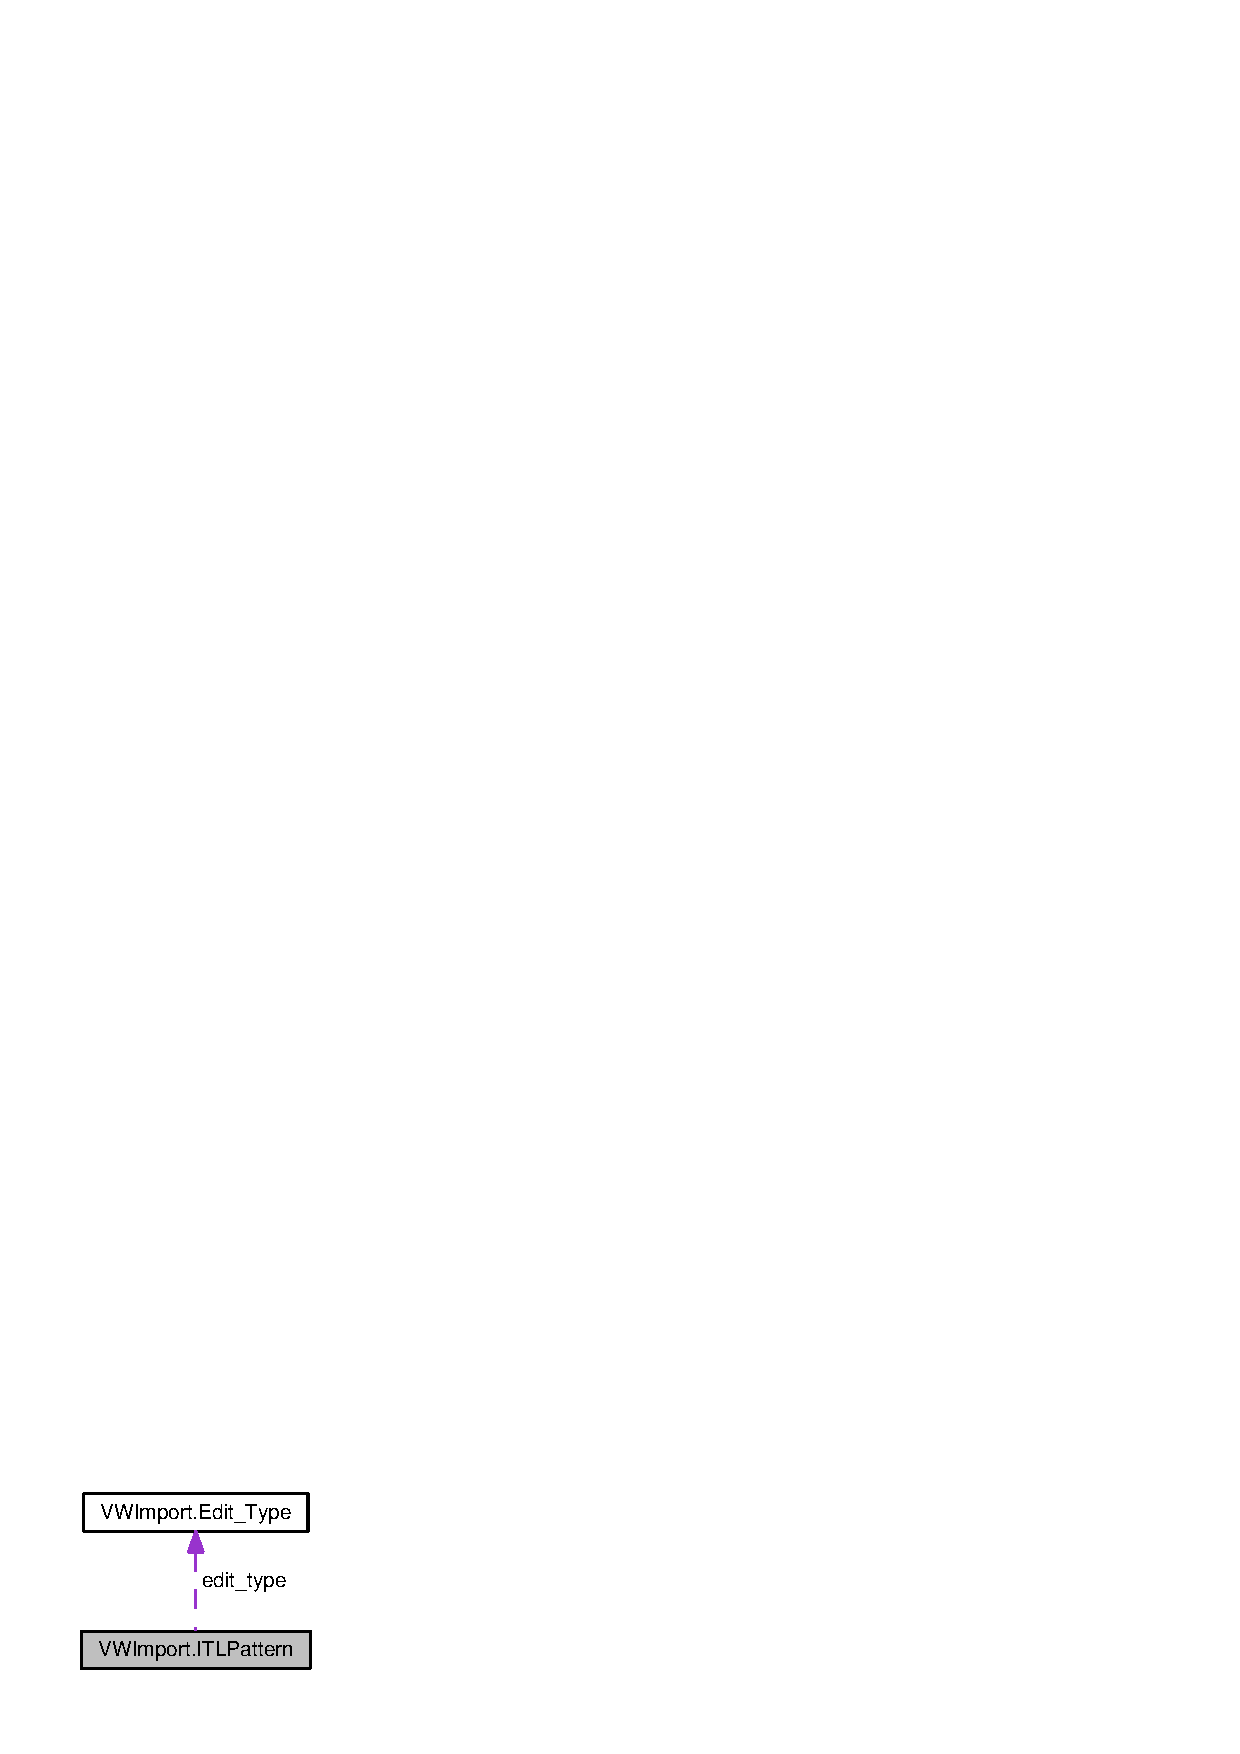
\includegraphics[width=152pt]{classorg_1_1smallfoot_1_1vw4_1_1VWImport_1_1ITLPattern__coll__graph}
\end{center}
\end{figure}
\subsection*{Data Fields}
\begin{DoxyCompactItemize}
\item 
{\bf Edit\-\_\-\-Type} {\bf edit\-\_\-type}\label{classorg_1_1smallfoot_1_1vw4_1_1VWImport_1_1ITLPattern_a76dab48266f34c941c947433ae14176d}

\begin{DoxyCompactList}\small\item\em What kind of edit are we doing? \end{DoxyCompactList}\item 
String {\bf initiator}\label{classorg_1_1smallfoot_1_1vw4_1_1VWImport_1_1ITLPattern_aecf64895f45b5dc828bdf693933ab6a7}

\begin{DoxyCompactList}\small\item\em initiator portion of the I\-T\-L pattern \end{DoxyCompactList}\item 
String {\bf lun}\label{classorg_1_1smallfoot_1_1vw4_1_1VWImport_1_1ITLPattern_ac6e080e7b7901a16bffc99d2ba56da3b}

\begin{DoxyCompactList}\small\item\em lun portion of the I\-T\-L pattern \end{DoxyCompactList}\item 
String {\bf target}\label{classorg_1_1smallfoot_1_1vw4_1_1VWImport_1_1ITLPattern_abeaebe344002fdda7a413305f5382548}

\begin{DoxyCompactList}\small\item\em target portion of the I\-T\-L pattern \end{DoxyCompactList}\end{DoxyCompactItemize}


\subsection{Detailed Description}
An \doxyref{I\-T\-L\-Pattern}{p.}{classorg_1_1smallfoot_1_1vw4_1_1VWImport_1_1ITLPattern} is udes to define an application \doxyref{Entity}{p.}{classorg_1_1smallfoot_1_1vw4_1_1VWImport_1_1Entity} based on the I\-T\-Ls it requires. 

For example an \char`\"{}\-Uber\-Database\char`\"{} application may define certain servers using certain L\-U\-Ns on certain storage targets 

Definition at line 36 of file V\-W\-Import.\-java.



The documentation for this class was generated from the following file\-:\begin{DoxyCompactItemize}
\item 
java/{\bf V\-W\-Import.\-java}\end{DoxyCompactItemize}

\section{V\+W\+Import Class Reference}
\label{classorg_1_1smallfoot_1_1vw4_1_1VWImport}\index{V\+W\+Import@{V\+W\+Import}}


A \doxyref{V\+W\+Import}{p.}{classorg_1_1smallfoot_1_1vw4_1_1VWImport} is a single idempotent import for the Virtual\+Wisdom4 product.  




Collaboration diagram for V\+W\+Import\+:\nopagebreak
\begin{figure}[H]
\begin{center}
\leavevmode
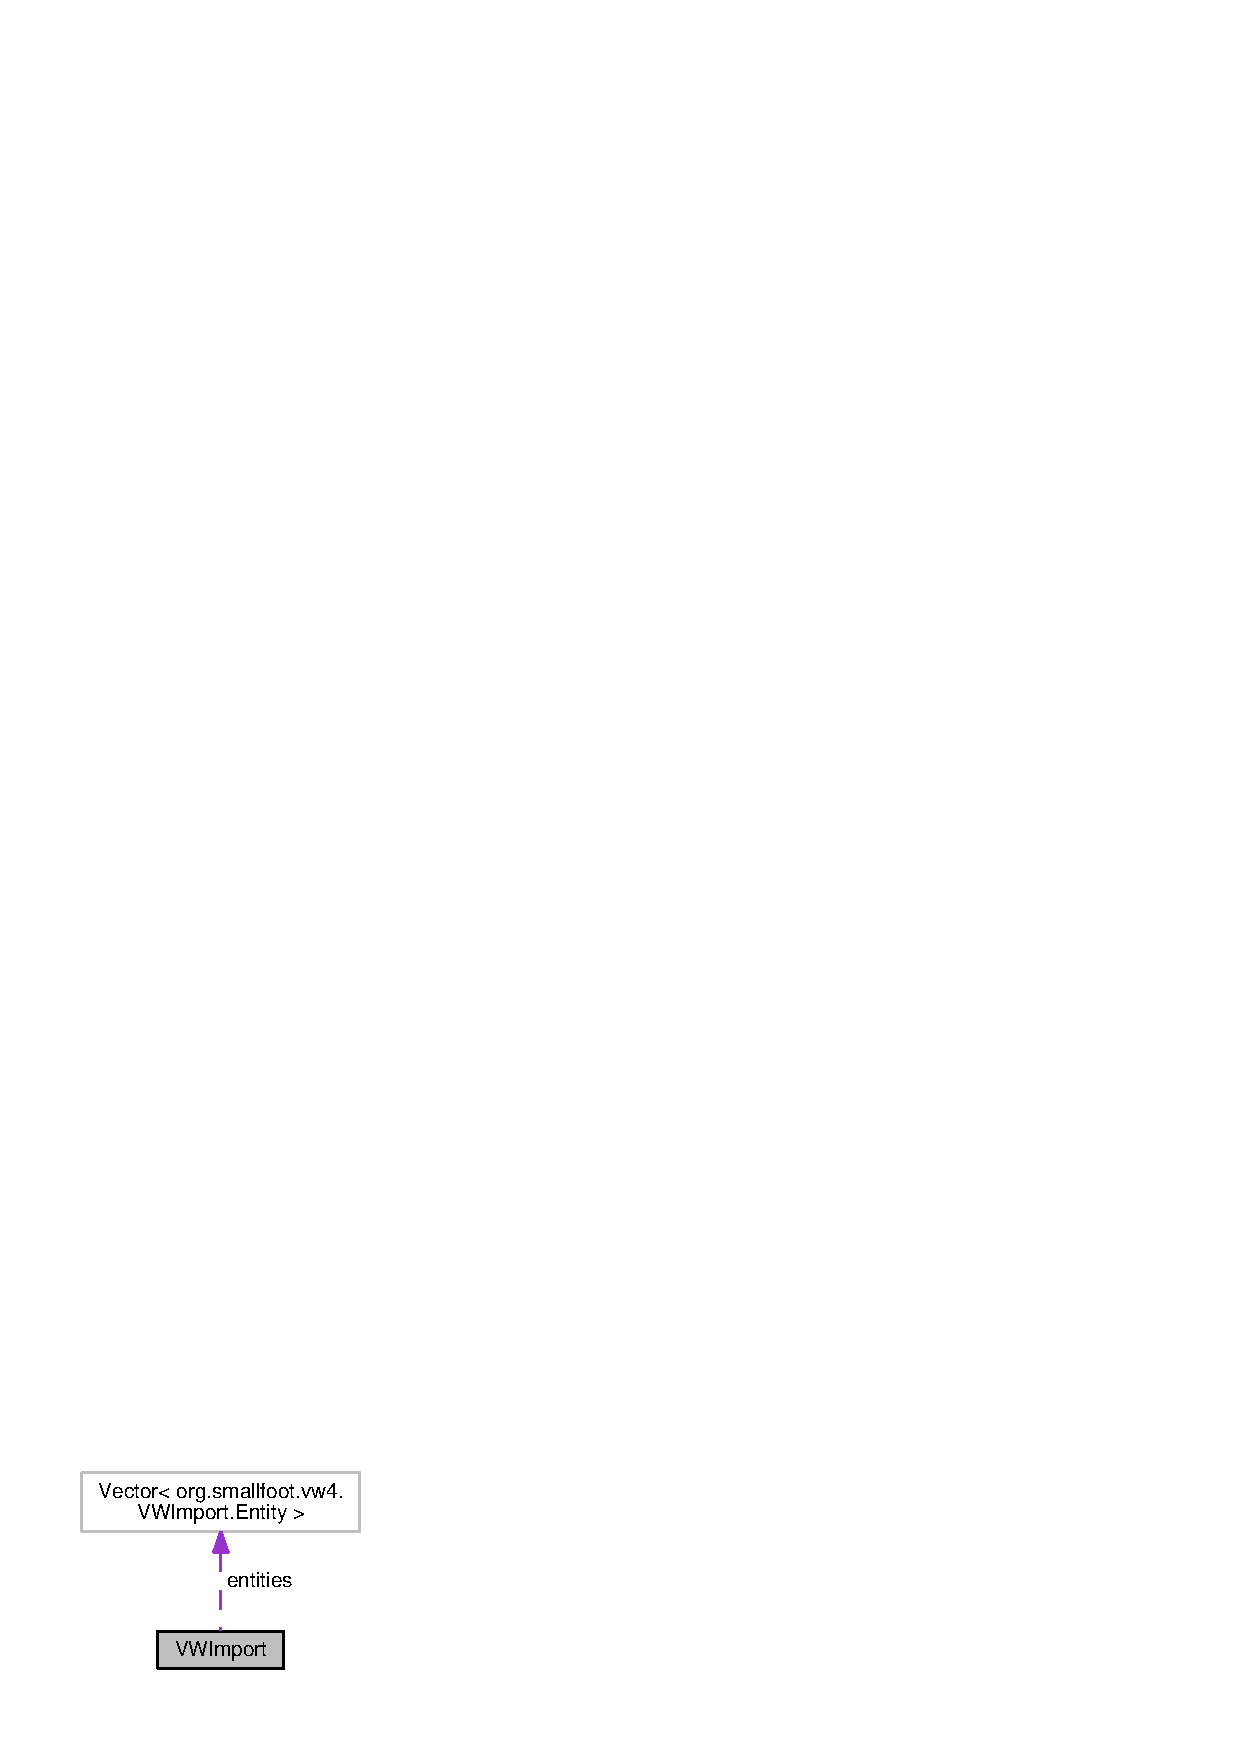
\includegraphics[width=176pt]{classorg_1_1smallfoot_1_1vw4_1_1VWImport__coll__graph}
\end{center}
\end{figure}
\subsection*{Data Structures}
\begin{DoxyCompactItemize}
\item 
enum {\bf Edit\+\_\+\+Type}
\begin{DoxyCompactList}\small\item\em The edit type of a J\+S\+O\+N for V\+W4 Import can be either \char`\"{}add\char`\"{} or \char`\"{}modify\char`\"{}; the creator needs to know ahead of time whether an entry of the same name currently exists. \end{DoxyCompactList}\item 
class {\bf Entity}
\begin{DoxyCompactList}\small\item\em An entity for import. \end{DoxyCompactList}\item 
class {\bf I\+T\+L\+Pattern}
\begin{DoxyCompactList}\small\item\em An \doxyref{I\+T\+L\+Pattern}{p.}{classorg_1_1smallfoot_1_1vw4_1_1VWImport_1_1ITLPattern} is used to define an application \doxyref{Entity}{p.}{classorg_1_1smallfoot_1_1vw4_1_1VWImport_1_1Entity} based on the I\+T\+Ls it requires. \end{DoxyCompactList}\item 
class {\bf Leaf\+Pattern}
\begin{DoxyCompactList}\small\item\em An \doxyref{Leaf\+Pattern}{p.}{classorg_1_1smallfoot_1_1vw4_1_1VWImport_1_1LeafPattern} is used to define an \doxyref{Entity}{p.}{classorg_1_1smallfoot_1_1vw4_1_1VWImport_1_1Entity} by reference in another entity's child\+\_\+entities. \end{DoxyCompactList}\end{DoxyCompactItemize}
\subsection*{Public Member Functions}
\begin{DoxyCompactItemize}
\item 
void {\bf add\+Entity} ({\bf Entity} e)\label{classorg_1_1smallfoot_1_1vw4_1_1VWImport_a20861f6c6a6268428f83e581368540c5}

\begin{DoxyCompactList}\small\item\em somewhat protected access / convenience method to append new entities \end{DoxyCompactList}\item 
Vector$<$ {\bf Entity} $>$ {\bf entities} ()\label{classorg_1_1smallfoot_1_1vw4_1_1VWImport_a66e795032db830396eddba947597ac21}

\begin{DoxyCompactList}\small\item\em singleton to provide an entity vector without having to check whether it's been created yet \end{DoxyCompactList}\item 
String {\bf get\+Version} ()\label{classorg_1_1smallfoot_1_1vw4_1_1VWImport_a12b5671e8920e8ce5c4457ea8d0d9fb2}

\begin{DoxyCompactList}\small\item\em it's great that the import format is versioned hence extensible, perhaps when some real-\/life-\/testing highlights concerns we've discussed \end{DoxyCompactList}\end{DoxyCompactItemize}
\subsection*{Protected Attributes}
\begin{DoxyCompactItemize}
\item 
Vector$<$ {\bf Entity} $>$ {\bf entities} = null\label{classorg_1_1smallfoot_1_1vw4_1_1VWImport_a9a3cd7caed5bd4b81c9383fc0e3c6e6f}

\begin{DoxyCompactList}\small\item\em the entities in the single Import action \end{DoxyCompactList}\end{DoxyCompactItemize}


\subsection{Detailed Description}
A \doxyref{V\+W\+Import}{p.}{classorg_1_1smallfoot_1_1vw4_1_1VWImport} is a single idempotent import for the Virtual\+Wisdom4 product. 

It's basically a wrapper for a number of entities and a version to define the format of the enclosed entities for import.

As a convention, Product Management recommends tagging all imported entities with \char`\"{}import\char`\"{} so that a select group can be dropped in case of errors rather than deleting all entities in the entire Virtual\+Wisdom product. 

Definition at line 17 of file V\+W\+Import.\+java.



The documentation for this class was generated from the following file\+:\begin{DoxyCompactItemize}
\item 
java/{\bf V\+W\+Import.\+java}\end{DoxyCompactItemize}

\chapter{File Documentation}
\section{htdocs/\-R\-E\-A\-D\-M\-E.dox File Reference}
\label{README_8dox}\index{htdocs/\-R\-E\-A\-D\-M\-E.\-dox@{htdocs/\-R\-E\-A\-D\-M\-E.\-dox}}

\section{java/\-V\-W\-Import.java File Reference}
\label{VWImport_8java}\index{java/\-V\-W\-Import.\-java@{java/\-V\-W\-Import.\-java}}
\subsection*{Data Structures}
\begin{DoxyCompactItemize}
\item 
enum {\bf V\-W\-Import.\-Edit\-\_\-\-Type}
\begin{DoxyCompactList}\small\item\em The edit type of a J\-S\-O\-N for V\-W4 Import can be either \char`\"{}add\char`\"{} or \char`\"{}modify\char`\"{}; the creator needs to know ahead of time whether an entry of the same name currently exists. \end{DoxyCompactList}\item 
class {\bf V\-W\-Import.\-Entity}
\begin{DoxyCompactList}\small\item\em An entity for import. \end{DoxyCompactList}\item 
class {\bf V\-W\-Import.\-I\-T\-L\-Pattern}
\begin{DoxyCompactList}\small\item\em An \doxyref{I\-T\-L\-Pattern}{p.}{classorg_1_1smallfoot_1_1vw4_1_1VWImport_1_1ITLPattern} is udes to define an application \doxyref{Entity}{p.}{classorg_1_1smallfoot_1_1vw4_1_1VWImport_1_1Entity} based on the I\-T\-Ls it requires. \end{DoxyCompactList}\item 
class {\bf V\-W\-Import}
\begin{DoxyCompactList}\small\item\em A \doxyref{V\-W\-Import}{p.}{classorg_1_1smallfoot_1_1vw4_1_1VWImport} is a single idempotent import for the Virtual\-Wisdom4 product. \end{DoxyCompactList}\end{DoxyCompactItemize}

%--- End generated contents ---

% Index
\newpage
\phantomsection
\addcontentsline{toc}{chapter}{Index}
\printindex

\end{document}
